\documentclass[a4paper,12pt]{report}


\usepackage[ngerman]{babel}
\usepackage[utf8]{inputenc}
\usepackage{blindtext}
\usepackage{graphicx}
\usepackage{amsmath}
\usepackage[onehalfspacing]{setspace}
\usepackage{pdfpages}
\usepackage{abstract}

\makeatletter
\renewenvironment{abstract}{%
    \if@twocolumn
      \section*{\abstractname}%
    \else %% <- here I've removed \small
      \begin{center}%
        {\bfseries \LARGE\abstractname\vspace{\z@}}%  %% <- here I've added \Large
      \end{center}%
      \quotation
    \fi}
    {\if@twocolumn\else\endquotation\fi}
\makeatother


%minimale page header & footer
\usepackage{fancyhdr}
\pagestyle{fancy}
\setlength{\headheight}{14pt} 
\fancyhf{}
\fancyhead[C]{\nouppercase{\leftmark}}
\fancyfoot[C]{\thepage}

%create links in the pdf
\usepackage[colorlinks]{hyperref}

\begin{document}
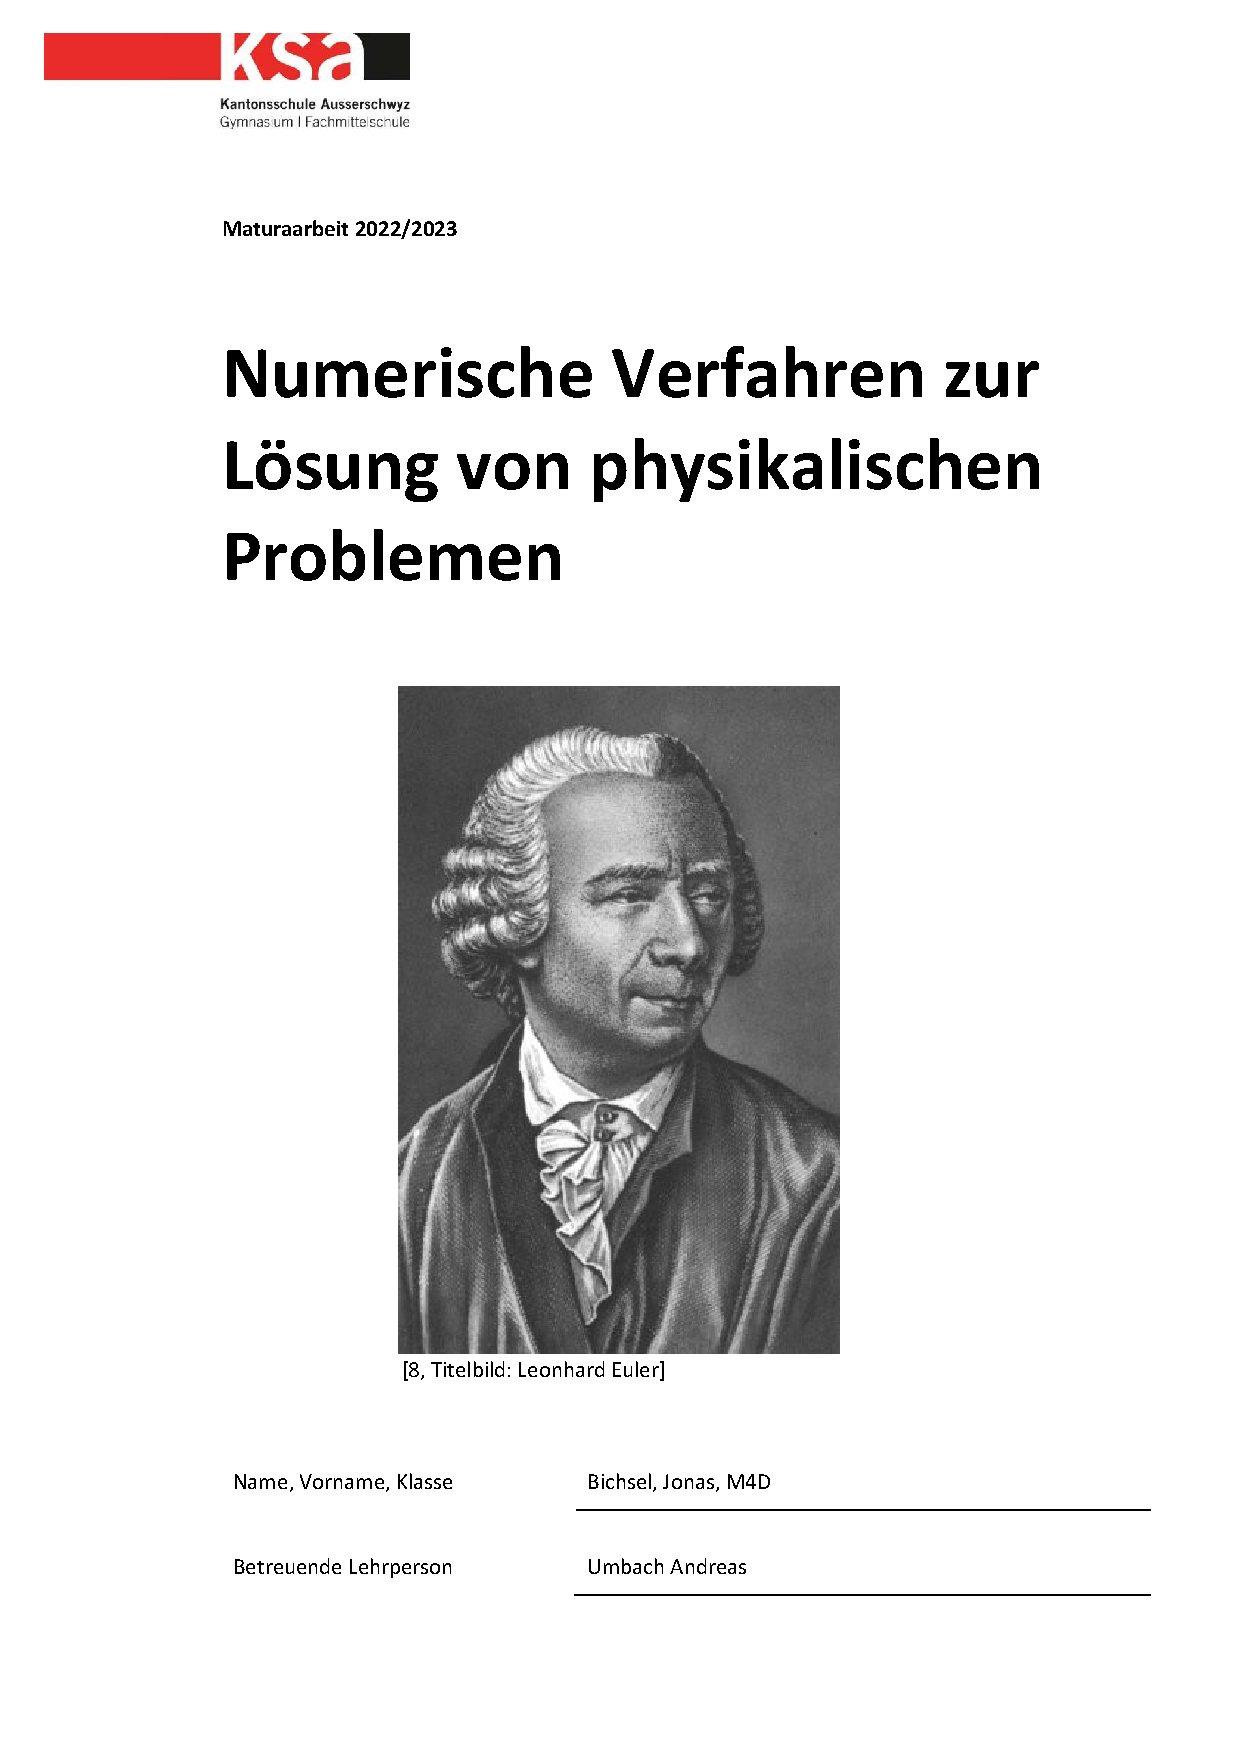
\includepdf{Ma_Titelblatt}
\begin{abstract}
\noindent
Die Physik ist eine wichtige Naturwissenschaft, welche die grundlegenden Phänomene der Natur untersucht. Ein wichtiger Bestandteil der Physik sind hierbei aufwendige Berechnungen, wie zum Beispiel die Berechnung der Umlaufbahn eines Planeten. Wie löst man nun Rechnungen, die zu komplex werden? Hierzu gibt es numerische Verfahren. In meiner Arbeit befasse ich mich mit drei numerischen Verfahren: eines zur Nullstellenbestimmung einer Funktion, dem Newton-Verfahren und zwei Methoden zur Lösung Differentialgleichungen, dem expliziten Euler-Verfahren und dem Verfahren von Heun. Alle drei Verfahren sind Näherungsverfahren, welche keine exakte Lösung liefern, sondern eine Approximation. Ich habe die Verfahren an physikalischen Problemen angewendet, für die ich exakte Lösungen hatte und dann die approximierten Lösungen mit den exakten verglichen. Dabei haben die numerischen Verfahren gut abgeschnitten. 
\end{abstract}
\tableofcontents


\chapter{Vorwort}
Ich bin schon seit längeren an Mathematik und Physik interessiert, darum wollte ich auch eine Maturaarbeit in einem dieser Fächer schreiben. Meine erste Idee war es, mich mit dem schiefen Wurf mit Luftwiderstand zu beschäftigen. Als ich damit zu meiner Betreuungsperson ging, kam Herr Umbach auf die Idee, das Thema auf numerische Verfahren zur Lösung von physikalischen Problemen zu erweitern. Ich fand diese Idee gut und so kam ich auf das Thema meiner Arbeit. An dieser Stelle möchte ich mich auch noch bedanken bei  meiner Betreuungsperson Andreas Umbach für seine Unterstützung und  bei meinen Eltern für das Gegenlesen der Arbeit.

\chapter{Einleitung}
In der Physik trifft man oft auf Berechnungen, sei es einfache Bewegungsgleichungen oder kompliziertere Umlaufbahnen eines Satelliten. Für das letztere reicht das Einsetzen von Variablen und einfache Rechnungen nicht mehr, hier kommen numerische Verfahren zum Spiel.\\

\noindent
Numerische Verfahren gibt es für verschiedene Probleme wie zum Beispiel lineare Gleichungssysteme oder Differentialgleichungen und auch schon für Differentialgleichungen gibt es viele verschiedene Verfahren. \\

\noindent
In der Arbeit schauen wir uns das explizite Euler-Verfahren und das Verfahren von Heun an und wenden sie bei der Entleerung von Staudämmen an. Ausserdem schauen wir uns das Newton-Verfahren zur Nullstellenbestimmung an.

\chapter{Numerik}
\section{Was ist numerische Mathematik}
Die numerische Mathematik ist ein Teilgebiet der Mathematik, welches sich mit der Konstruktion und Analyse von Algorithmen zur Lösung von mathematischen Problemen befasst. Ziel der Numerik ist die Konstruktion von möglichst effizienten und stabilen Algorithmen. Diese Algorithmen (numerische Verfahren) kommen dann zum Zug, wenn es keine explizite Lösungs-darstellung gibt oder wenn die Lösungsdarstellung zu kompliziert ist und somit nicht geeignet, um schnell an ein Ergebnis zu kommen. Mathematische Probleme bei denen numerische Verfahren angewendet werden, kommen zum Beispiel aus der Physik, Technik, Ökonomie usw.. \cite[Harbrecht S.5]{Harbrecht} \cite[Numerik-Mathepedia]{Mathepedia} \\

\noindent
Generell werden zwei Typen von Verfahren unterschieden. Der direkte Typ, welcher nach einer endlichen Zeitspanne ein exaktes Resultat für ein Problem liefert. Darunter fällt zum Beispiel der erweiterte euklidische Algorithmus. Der zweite Typ sind Näherungsverfahren, welche keine exakte Lösung berechnen, sondern nur eine Approximation liefern. Das Newton-Verfahren \ref{Newton}, welches zum Approximieren einer Nullstelle gebraucht wird, ist so ein numerisches Verfahren. \cite[Numerik-Mathepedia]{Mathepedia}

\section{Beispiel: Newton-Verfahren} \label{Newton}
Das Newton-Verfahren ist ein gutes Beispiel für ein einfaches, numerisches Verfahren. Hierbei handelt es sich um ein Algorithmus zur numerischen Bestimmung einer Nullstelle. Es ist ein iteratives, bei dem man mit einem Startwert $x_0$ beginnt und so $x_n$ berechnet, je mehr Schritte man macht, desto genauer wird das Resultat. Mit diesem Verfahren kann man relativ schnell die Nullstelle approximieren. Jedoch kann es bei einem ungünstig gewählten Startwert dazu kommen, dass man die Nullstelle nicht approximieren kann. \cite[StudyHelp]{Newton-Verfahren}
\noindent
Für das Newton-Verfahren gilt: 
\begin{equation*}
1.Schritt: x_1 = x_0 - \frac{f(x_0)}{f'(x_0)}
\end{equation*}

\begin{equation*}
n-ter Schritt: x_n = x_{n-1} - \frac{f(x_{n-1})}{f'(x_{n-1})}
\end{equation*}

\subsection{Herleitung}
Die Grundidee hinter dem Newton-Verfahren ist, dass wenn man ein Punkt f($x_0$) auf einer Funktion nimmt, schaut, wo die Tangente dieses Punktes die x-Achse schneidet und dann den x-Wert des Schnittpunktes mit $x_0$ vergleicht, ist der neue x-Wert ($x_1$) näher an der Nullstelle als $x_0$. Wenn man jetzt mit $x_1$ das Ganze repetiert und immer so weiter,  nähert man sich der Nullstelle. Wir beginnen somit bei der Herleitung mit der Tangentengleichung:
 \begin{equation}
t(x) = mx + n
\end{equation}
Hierbei ist m die Steigung der Tangente und n ist die Stelle, an der die Tangente die y-Achse schneidet (y-Achsenabschnitt). Da unsere Tangente an der Stelle f($x_0$) anliegt, ist die Steigung der Tangente gleich der ersten Ableitung von f(x) an der Stelle $x_0$:
 \begin{equation}
t(x) = f'(x_0) \cdot  x + n
\end{equation}
Um n zu bestimmen, setzen wir nun $x_0$ in t(x) ein. Da die Tangente f(x) am Punkt ($x_0$\big \vert f($x_0$)) berührt ist t($x_0$) = f($x_0$):
 \begin{equation}
f(x_0) = f'(x_0) \cdot x_0 + n
\end{equation}
Wenn wir die Gleichung nun auf n Auflösen erhalten wir: 
\begin{equation}
n = f(x_0) -  f'(x_0) \cdot x_0
\end{equation}
Nun setzen wir den Term, welchen wir für n erhalten haben, in t(x) ein: 
 \begin{equation}
t(x) =  f'(x_0) \cdot x + f(x_0) -  f'(x_0) \cdot x_0
\end{equation}
Jetzt können wir die Nullstelle $x_1$ der Tangente berechnen. Dafür setzen wir $x_1$ in t(x) ein und setzen den Term gleich null, da er die y-Achse schneidet: 
 \begin{equation}
t(x_1) =  f'(x_0) \cdot x_1 + f(x_0) -  f'(x_0) \cdot x_0 = 0 
\end{equation}
Wenn man nun die Gleichung auf $x_1$ auflöst erhält man das Newton-Verfahren: 
\begin{equation}
x_1 = x_0 - \frac{f(x_0)}{f'(x_0)}
\end{equation}

\subsection{Anwendungsbeispiel}
Nachdem wir das Newton-Verfahren hergeleitet haben, überprüfen wir nun, wie gut das Verfahren ist. Hierzu nehmen wir ein Rechenbeispiel, welches eine exakte Lösung hat, damit wir dieses Ergebnis mit den Approximationen des Newton-Verfahrens vergleichen können. Als Beispiel nehmen wir den schiefen Wurf ohne Luftwiderstand und möchten herausfinden, welche horizontale Distanz ein Körper mit der Geschwindigkeit 10m/s und dem Abschusswinkel 45° zurücklegt, bevor er wieder auf dem Boden aufkommt.
Für den schiefen Wurf gilt:
\begin{equation*}
f(x) = tan(\alpha) \cdot x - \frac{1}{2} \cdot \frac{g}{v_{0}^{2} \cdot cos^2(\alpha)} \cdot x^2
\end{equation*}
Wobei g die Erdbeschleunigung (9.81m/$s^2$) ist, $v_0$ die Geschwindigkeit (10m/s) und $\alpha$ der Abschusswinkel (45°). Wenn wir den Term nun gleich null setzen und x ausrechnen, erhalten wir zwei Lösungen. Einmal x = 0, weil der Gegenstand sich beim Start auf dem Boden befindet und einmal x $\approx $ 10.19368, welches die gesuchte Distanz ist.
Wenn wir nun das Newton-Verfahren anwenden mit einem Startwert von $x_0 = 8$ dann erhalten wir folgende Resultate:\\


\begin{center}
\begin{tabular}[h]{c|c}

$x_n$ & Wert \\
\hline
$x_0$ & 8 \\
\hline 
$x_1$ & 11,02247 \\
\hline
$x_2$ & 10,25163 \\
\hline
$x_3$ & 10,19400 \\
\hline
$x_4$ & 10,19368\\

\end{tabular}
\end{center}


\noindent
\\Wenn man nun die Werte der Tabelle mit dem auf fünf Nachkommastellen gerundeten Wert (x $\approx $ 10.19368) vergleicht, können wir sehen, dass das Newton-Verfahren bereits nach drei Durchgängen schon auf drei Nachkommastellen genau und nach vier auf fünf genau ist. \\

\noindent
Anhand dieses Beispiels ist gut ersichtlich, wie das Newton-Verfahren schon nach wenigen Durchgängen extrem nahe an das exakte Resultat herankommt. 

\chapter{Numerik bei Differentialgleichungen}
\section{Differentialgleichungen}
Bei Differentialgleichungen handelt es sich um mathematische Gleichungen, bei denen man nicht eine oder mehrere Zahlen sucht, sondern eine Funktion. In der Physik spielen Differentialgleichungen eine wichtige Rolle, da man viele physikalische Gesetze und Zusammenhänge mit Differentialgleichungen darstellen kann. Bereits Geschwindigkeit und Beschleunigung sind nichts anderes als die erste, respektive die zweite Ableitung der Strecke nach der Zeit: $s(t)' = v \vert s(t)'' = a$. Wenn eine Ableitung und deren Funktion in einer Gleichung vorkommt, spricht man von einer Differentialgleichung. Die Ordnung der Differentialgleichung richtet sich nach der höchsten Ableitung. Man unterscheidet auch zwischen linearen und nicht-linearen Differentialgleichungen. Eine Differentialgleichung ist dann linear, wenn die Funktion und deren Ableitung linear sind, das heisst sie haben die Potenz 1. Eine lineare Differentialgleichung wäre zum Beispiel: $y' = y + x$ und eine nicht-lineare: $y' = \sqrt{y}+ x$. In der Regel gibt es unendlich viel Lösungen für eine Differentialgleichung. Um die Lösungsmenge einzugrenzen, gibt man entweder $y(x)'$ oder $y(x)$ eine Bedingung, wie zum Beispiel $y(0) = 0$. In der Physik trifft man meistens auf Differentialgleichungen erster oder zweiter Ordnung und viel davon sind linear. Für das Lösen von Differentialgleichungen gibt es auch numerische Verfahren, wie das Euler-Verfahren \ref{Euler} oder das Verfahren von Heun \ref{Heun}. \cite[Spektrum.de]{Differentialgleichung}

\section{Explizites Euler-Verfahren}\label{Euler}
Das explizite Euler-Verfahren ist das einfachste, numerische Verfahren für Anfangswertprobleme. Anfangswertproblem sind Differentialgleichungen mit einem Anfangswert als zusätzliche Bedingung. Für Anfangswert Probleme braucht man also eine Differentialgleichung: $y'(x) = f(x, y(x))$, einen Anfangsbedingung: $y(x_0) = y_0$, $x_0$ und $y_0$ sind hier vorgegebene Werte. Die Idee des expliziten Euler-Verfahren ist es durch die Steigung an einem Punkt den nächsten y-Wert zu approximieren. Da die Steigung definiert ist als: $m = \frac{\Delta y}{\Delta x}$ gilt: $\Delta y = \Delta x \cdot m$. Wenn wir eine lineare Funktion hätten, könnten wir nun einfach hiermit das $\Delta y$ für ein $\Delta x$ berechnen. Nur handelt es sich im Normalfall nicht um eine lineare Funktion, die an allen Punkten die gleiche Steigung hat.\\

\noindent
Euler kam nun aber auf die Idee: Er beginnt bei $x_0\vert y_0$ mit einer Schrittweite von h. Für diesen h grossen Abschnitt behandelt er die Funktion wie eine lineare Funktion, um so den neuen y-Wert zu approximieren. Danach nimmt man den neuen y-Wert und macht dort mit der neuen Steigung das Gleiche.

\begin{equation*}
x_k = x_0 + kh, (k = 1, 2, ...)
\end{equation*}
\begin{equation*}
y_{k+1} = y_k + hf(x_k, y_k),	(k= 1, 2, ...)
\end{equation*}

\noindent
\\Nehmen wir als Beispiel mal $x_0 = 0, y_0 = 0$ und eine Schrittweite h = 0.1, dann sagt man mit dem expliziten Euler-Verfahren, dass die Steigung zwischen x = 0 und x = 0.1 gleich der Steigung am Punkt $(0\vert0)$ ist und approximiert dann so den y-Wert für x = 0.1. Als nächsten Schritt sagt man, dass die Steigung zwischen x = 0.1 und x = 0.2 gleich der Steigung am neuen Punkt ist und approximiert so den y-Wert an x = 0.2 und so weiter. Die Genauigkeit des expliziten Euler-Verfahrens ist von der Schrittweite h abhängig. Je grösser h, desto ungenauer ist das Verfahren. Um mehr über die Genauigkeit zu erfahren, schauen wir uns die Taylorreihe an. Durch die Taylorreihe kann man auch den Wert einer Funktion an einem Punkt approximieren, wenn man die Ableitungen der Funktion und einen Startwert hat. Bei der Taylorreihe handelt es sich um eine unendlich lange Polynomreihe.
\begin{equation*}
y(x + \Delta x) = y(x) + (\Delta x) \cdot y'(x) + \frac{\Delta x^2}{2!} \cdot y''(x) + \frac{\Delta x^3}{3!} \cdot y'''(x) +... 
\end{equation*}
Wenn man die Taylorreihe mit dem expliziten Euler-Verfahren vergleicht, sieht man, dass der erste Summand der Taylorreihe gleich dem expliziten Euler-Verfahren ist. Demnach ist der ganze Rest der Taylorreihe gleich dem Fehler des expliziten Euler-Verfahrens und somit hat das explizite Euler-Verfahren einen Fehler der Ordnung O($h^2$). Der Fehler mag zwar immens klingen, doch wenn man mit einer Schrittweite h=0.1 arbeitet, ist er nicht mehr so gross. Im Kapitel \ref{Staudam} wenden wir das Verfahren auch noch an um den Fehler an einem konkreten Beispiel zu sehen. \cite[Bourg S. 174-180]{Bourg} \cite[Schwarz S. 413-419]{Schwarz}

\section{Verfahren von Heun}\label{Heun}
Durch das Vergleichen des expliziten Euler-Verfahrens mit der Taylorreihe haben wir gesehen, wie das explizite Euler-Verfahren nur aus dem ersten Summanden der Taylorreihe besteht und der Rest der Reihe ist Fehler. Jedoch gibt es auch noch genauere Verfahren, eins davon ist das Verfahren von Heun mit einem Fehler der Ordnung O($h^3$). Die Grundidee des Verfahrens von Heun ist die gleich wie die beim expliziten Euler-Verfahren aber mit einem entscheidenden Unterschied. Das Verfahren von Heun braucht nicht nur die Steigung $f(x_0, y_0)$, wie beim expliziten Euler-Verfahren, sondern nimmt auch noch die Steigung $f(x_1, y_1)$ dazu, berechnet den Durchschnitt der beiden Steigungen und rechnet dann mit diesem Durchschnitt genau gleich wie beim expliziten Euler-Verfahren.
\begin{equation*}
y_{k+1} = y_k + \frac{h}{2}(f(x_k, y_k) + f(x_{k+1}, y_{k+1}))
\end{equation*}
Bei der Gleichung gibt es jedoch ein grosses Problem, denn um die Gleichung lösen zu können, braucht man bereits die Lösung der Gleichung. Wenn man die Lösung der Gleichung nicht hat, wie soll man dann die Gleichung lösen und wenn man sie hat, warum sollte man dann die Gleichung nochmals lösen? Hier berechnen wir aber keine exakte Lösung, sondern approximieren nur einen Wert. Der Sinn des Verfahrens von Heun ist, exakter zu sein, als das explizite Euler-Verfahren. Also approximiert man zuerst $y_{k+1}$ durch das explizite Euler-Verfahren und setzt dann diesen Wert im Verfahren von Heun ein, um eine genauere Approximation zu erhalten. \cite[Schwarz S.420-424]{Schwarz}

\chapter{Entleerung eines Staudammes}\label{Staudam}
\section{Theorie}
Da wir nun zwei numerische Verfahren für Differentialgleichungen kennen, wollen wir diese nun anwenden. Hierzu betrachten wir den Ausfluss eines Staudammes mit rechteckigen Längsschnitt, eines mit dreieckigem Längssch- nitt und einer umgekehrten Pyramide. Hierbei wollen wir die Höhe des Wasserstandes zu einem bestimmten Zeitpunkt berechnen können. Der Vorteil dieses Beispieles ist, dass es eine exakte Lösung gibt und wir diese mit der Lösung des expliziten Euler-Verfahrens und des Verfahrens von Heun vergleichen können. Um die Höhenveränderung zu kennen, müssen wir zuerst wissen, mit welcher Geschwindigkeit das Wasser unseren Staudamm verlässt. Hierzu nehmen wir Gebrauch von der Energieerhaltung. Beim entleeren wird die Lageenergie des Wassers in kinetische Energie umgewandelt. Die Lageenergie (potenzielle Energie) ist abhängig von der Lage eines Körpers, das heisst je höher der Körper, desto grösser die Lageenergie. Da die Lageenergie zur kinetischen Energie umgewandelt wird, müssen beide Energien gleich gross sein:
\begin{equation}
W_{pot} = W_{kin}
\end{equation} 
\begin{equation}
m \cdot g \cdot h = \frac{1}{2} \cdot m \cdot v_a^2
\end{equation} 
Wenn wir die Gleichung nun nach der Ausflussgeschwindigkeit ($v_a^2$) umformen, erhalten wir die Formel für die Ausflussgeschwindigkeit: 
\begin{equation} \label{va}
v_a = \sqrt{2gh}
\end{equation} 
Anhand dieser Formel können wir nun sehen, dass die Ausflussgeschwindigkeit nur vom Höhenunterschied zwischen der Oberfläche der Flüssigkeit und der Öffnung abhängig ist. Sie ist ausserdem nicht von der Dichte abhängig, sofern man die Reibung vernachlässigt, somit ist egal, ob wir Wasser oder eine andere Flüssigkeit in unserem Staudamm haben. Die Ausflussgeschwindigkeit alleine hilft uns aber noch nicht so viel, da wir damit noch nicht die Entleerungszeit bestimmen können, denn diese ist auch abhängig von der Form und Grösse des Gefässes und der Öffnung. Hierzu betrachten wir zuerst ein Gefäss mit einem konstanten Querschnitt (A), die Flüssigkeit fliesst am Boden durch ein Loch mit dem Querschnitt $A_a$. Um jetzt die Endleerungszeit herauszufinden, müssen wir einen Zusammenhang zwischen ihr und der Ausflussgeschwindigkeit finden. Hierbei hilft uns die Massenerhaltung, welche besagt, dass die Masse des Wassers, welches unten herausströmt, der Masse, um die der Behälter abnimmt, entspricht und somit verringert sich das Flüssigkeitsvolumen im Körper um genau das ausströmende Volumen. Das abgenommene Volumen im Körper entspricht dem Querschnitt mal den Höhenunterschied und das ausströmende Volumen entspricht der Strecke, welches das Wasser zurücklegt, $v_a \cdot \Delta t$ mal den Öffnungsquerschnitt. Somit gilt:
\begin{equation}
\Delta h \cdot A = v_a \cdot \Delta t \cdot A_a
\end{equation} 
Um die Zeit für das Entleeren herauszufinden, brauchen wir die Sinkgeschwindigkeit (v) im Körper. Da aber die Sinkgeschwindigkeit mal den Zeitunterschied den Höhenunterschied ergeben, können wir den Höhenunterschied ersetzen:
\begin{equation}
v \cdot \Delta t \cdot A = v_a \cdot \Delta t \cdot A_a
\end{equation} 
Wenn wir nun für $v_a$ unsere Formel \ref{va} einsetzen und die Gleichung auf v auflösen, haben wir die Formel für die Sinkgeschwindigkeit:
\begin{equation}
v = \frac{A_a}{A} \cdot \sqrt{2gh}
\end{equation} 
Wenn wir nun die Formel betrachten, sehen wir, dass die Sinkgeschwindigkeit von der Höhe abhängig ist, diese jedoch selbst verändert und somit selbst wieder auf ein anderes Resultat kommt. Die Sinkgeschwindigkeit ist jedoch nichts anderes als die Änderung der Füllstandshöhe (dh) pro Zeit (dt): 
\begin{equation}
v = - \frac{dh}{dt}
\end{equation} 
Das negative Vorzeichen ist da, weil bei positiver Sinkgeschwindigkeit sich die Höhe verringert. 
\begin{equation}
- \frac{dh}{dt} = \frac{A_a}{A} \cdot \sqrt{2gh}
\end{equation} 
Nun haben wir eine Differentialgleichung, welche wir mit dem expliziten Euler-Verfahren oder mit dem Verfahren von Heun lösen können. 
\begin{equation} \label{dd}
 h'(t)=- \frac{A_a \cdot  \sqrt{2g}}{A} \cdot \sqrt{h(t)}
\end{equation}
Die Funktion der exakten Lösung, mit welcher wir dann das Euler-Verfahren und das Verfahren von Heun vergleichen werden, lautet: 
\begin{equation}
h(t) = \left( \sqrt{H} - \frac{A_a}{A} \sqrt{\frac{g}{2}} \cdot t \right)^2
\end{equation}
H ist hier die Starthöhe. Wir haben jetzt die Differentialgleichung und Funktion für einen Körper, bei dem sich der Querschnitt nicht verändert. Bei einem Staudamm, mit einem dreieckigen Längsschnitt oder einer umgekehrten Pyramide, ist der Querschnitt aber auch von der Höhe abhängig. Bei einem dreieckigen Längsschnitt verändert sich der Querschnitt lineare, die Funktion dazu lautet:
\begin{equation}
A(h) = \frac{A_0}{H} \cdot h 
\end{equation} 
Wenn wir die Funktion nun in \ref{dd} für A einsetzen, erhalten wir die Differentialgleichung für einen dreieckigen Längsschnitt:
\begin{equation}\label{d2}
 h'(t)=- \frac{A_a \cdot  \sqrt{2g} \cdot H}{A_0} \cdot h(t)^{- \frac{1}{2}}
\end{equation}  
Dementsprechend verändert sich auch die Funktion für die exakte Lösung: 
\begin{equation}
h(t) = \left( H^{\frac{3}{2}}- \frac{3}{2} \cdot \frac{A_a \cdot  \sqrt{2g} \cdot H}{A_0} \cdot t \right)^{\frac{2}{3}}
\end{equation} 
Bei einer umgekehrten Pyramide verändert sich die Höhe nicht linear wie bei einem dreieckigen Längsschnitt, sondern quadratisch. Die Funktion dazu lautet: 
\begin{equation}
A(h) = \frac{A_0}{H^2} \cdot h^2 
\end{equation} 
Wenn wir diese Funktion nun wieder in \ref{dd} für A einsetzen, erhalten wir: 
\begin{equation}\label{d3}
 h'(t)=- \frac{A_a \cdot  \sqrt{2g} \cdot H^2}{A_0} \cdot h(t)^{- \frac{3}{2}}
\end{equation}
Somit ist die Funktion für eine umgekehrte Pyramide: 
\begin{equation}
h(t) = \left( H^{\frac{5}{2}}- \frac{5}{2} \cdot \frac{A_a \cdot  \sqrt{2g} \cdot H^2}{A_0} \cdot t \right)^{\frac{2}{5}}
\end{equation} \cite[Tec-science]{Tec-science}

\section{Berechnung}
Da wir nun die Differentialgleichungen haben und die dazugehörigen Funktionen, können wir das explizite Euler-Verfahren und das Verfahren von Heun mit der exakten Lösung vergleichen. Betrachten wir zuerst einen Staudamm mit einem rechteckigen Längsschnitt. Nehmen wir an, unser Staudamm hat eine Höhe von 1000 Meter und eine Querschnittsfläche von 100$m^2$, das ergibt ein Wasservolumen von 100'000$m^3$. Jetzt brauchen wir noch den Querschnitt des Abflussrohres, welcher 2$m^2$ ist. Die Funktion für unseren Staudamm lautet also:
\begin{equation}
h(t) = \left( \sqrt{1000} - \frac{2}{100} \sqrt{\frac{9.81}{2}} \cdot t \right)^2
\end{equation}
Nun brauchen wir noch die Gleichung für das explizite Euler-Verfahren und das Verfahren von Heun. Da wir bereits die Differentialgleichung haben und auch einen Startwert, denn bei Start der Entleerung ist der Staudamm voll, somit ist gilt $t_0 = 0$ und $h_0 = 1000$. Das explizite Euler-Verfahren kennen wir bereits aus Kapitel \ref{Euler}, wenn wir dies für unseren Staudamm umschreiben, wobei $h'(t)$ der Differentialgleichung \ref{dd} entspricht und wir mit einer Schrittweite von 1 rechnen:
\begin{equation}
h(t_1) = h_0 + 1 \cdot h'(t_0, h_0)
\end{equation}
Nun noch die Gleichung vom Verfahren von Heun, auch mit einer Schrittweite von 1: 
\begin{equation}
h(t_1) = h_0 + \frac{1}{2} (h'(t_0, h_0) + h'(t_1, h_1))
\end{equation}
Wenn man nun mit Hilfe des Computers die einzelnen Punkt ausrechnet erhält man diese Werte: \\

\begin{center}
\begin{tabular}[h]{c|c|c|c}
t & Exakte Lösung & explizites Euler-Verfahren & Verfahren von Heun \\
\hline
0 & 1000 & 1000 & 1000 \\
\hline
1 & 997.2005338 & 997.1985718 & 997.2005352 \\
\hline
2 & 994.4049916 & 994.4010703 & 994.4049957 \\
\hline
3 & 991.6133734 & 991.6074956 & 991.6133816 \\
\hline
10 & 972.1819179 & 972.1624222 & 972.1819938 \\
\hline
100 & 739.4771793 & 739.295274 & 739.4842922 \\
\hline
300 &336.1515378 & 335.7084679 & 336.2180772 \\
\hline
700 & 0.380254972 & 0.276602066 & 0.622374512 \\
\hline
709 & 0.047523107 & 0.00774161 & 0.247664522 \\

\end{tabular}
\end{center}

\noindent
\\Wenn man die Tabelle betrachtet, sieht man, dass zu Beginn das Verfahren von Heun bis auf fünf Nachkommastellen genau aus. Mit der Zeit nimmt diese Genauigkeit aber ab, da sich die ungenauen Zwischenresultate anhäufen. Bei diesem Beispiel ist das explizite Euler-Verfahren am Anfang ungenauer als das Verfahren von Heun, gegen den Schluss ist es aber genauer. Im Normalfall sollte das Verfahren von Heun eigentlich genauer sein, jedoch gibt es auch Ausnahmen dazu. Für das vollständige Entleeren des Staudammes braucht es 714 Sekunden. Excel konnte jedoch nur bis 709 Sekunden rechnen, da bei 710 Sekunden das explizite Euler-Verfahren bereits so nah an null dran war, sodass für den nächsten Schritt $0^{-\frac{1}{2}}$ ausgerechnet werden müsste, was jedoch in einer Division durch null enden würde. \\

\noindent
Als nächstens möchten wir noch schauen, wie gut die beiden Algorithmen bei einem Staudamm mit dreieckigem Längsschnitt und bei einer auf den Kopf gestellten Pyramide abschneiden und wir können auch die Entleerungszeit der drei Staudämme miteinander vergleichen. Damit wir aber die Entleerungszeit der drei Staudämme vergleichen können, brauchen alle das gleiche Volumen und damit wir die Veränderung der Höhe auch noch vergleichen können, sollen alle die gleiche Höhe haben. Damit nun der Staudamm mit dem dreieckigen Längsschnitt das gleiche Volumen hat, braucht er ein $A_0$ von $200m^2$. Somit lautet die Funktion für unseren Staudamm:
\begin{equation}
h(t) = \left( 1000^{\frac{3}{2}}- \frac{3}{2} \cdot \frac{2 \cdot  \sqrt{2g} \cdot 1000}{200} \cdot t \right)^{\frac{2}{3}}
\end{equation} 
Für das explizite Euler-Verfahren und das Verfahren von Heun gilt das gleiche wie beim vorherigen Staudamm, mit Ausnahme, dass $h'(t)$ jetzt wie bei \ref{d2} ist. Wenn man nun das Ganze wieder ausrechnet, erhält man folgende Resultate: \\

\begin{center}
\begin{tabular}[h]{c|c|c|c}
t & Exakte Lösung & explizites Euler-Verfahren & Verfahren von Heun \\
\hline
0 & 1000 & 1000 & 1000 \\
\hline
1 &998.5987949 & 998.5992859 & 998.5987949 \\
\hline
2 & 997.1966061 & 997.1975898 & 997.1966062 \\
\hline
3 & 995.7934308 & 995.7949088 & 995.7934311 \\
\hline
10 & 985.9433452 & 985.9483336 & 985.9433526 \\
\hline
100 & 854.5001325 & 854.559639 & 854.5012694 \\
\hline
200 & 695.3098271 & 695.4622419 & 695.3165008 \\
\hline
400 & 294.1961288 & 294.9827391 & 294.3049773 \\
\hline
476 & $\approx 0$ & 15.85441551 & 8.910568699 \\

\end{tabular}
\end{center}


\noindent
\\Nach gerundet 476 Sekunden ist dieser Staudamm leer, was deutlich schneller ist als unser vorheriger Staudamm mit 714 Sekunden. Wenn man hier wieder die exakten Werte mit den Werten von den beiden Verfahren vergleicht, sieht man, dass am Anfang die beiden Verfahren relativ exakt sind, gegen den Schluss verlieren sie aber an Genauigkeit, da sich die Steigung immer stärker verändert. Am Schluss ist, wie es eigentlich sein sollte, das Verfahren von Heun genauer als das explizite Euler-Verfahren. \\

\noindent
Zum Schluss schauen wir uns noch die Entleerungszeit einer auf den Kopf gestellten Pyramide an. Damit die Pyramide mit gleicher Höhe trotzdem das gleiche Volumen hat, muss der Startquerschnitt dreimal so gross sein wie bei unserem ersten Staudamm. Dies kann man aus der Formel für das Volumen einer Pyramide herauslesen: $V = \frac{1}{3} \cdot h \cdot A_0$. Somit muss $A_0$ $300 m^2$ gross sein, damit die Pyramide das gleiche Volumen wie die beiden andern Staudämme hat. Die Funktion dafür lautet:
\begin{equation}
h(t) = \left( 1000^{\frac{5}{2}}- \frac{5}{2} \cdot \frac{2 \cdot  \sqrt{2g} \cdot 1000^2}{300} \cdot t \right)^{\frac{2}{5}}
\end{equation} 
Beim Euler-Verfahren und dem Verfahren von Heun ändert sich wieder nur $h'(t)$ zu Steigung bei \ref{d3}. Nun berechnen wir die Werte wieder mit dem Computer. \\

\begin{center}
\begin{tabular}[h]{c|c|c|c}
t & Exakte Lösung & explizites Euler-Verfahren & Verfahren von Heun \\
\hline
0 & 1000 & 1000 & 1000 \\
\hline
1 &999.0655358 & 999.0661906& 999.0655358 \\
\hline
2 & 998.1297587 & 998.1310717 & 998.1297592\\
\hline
3 & 997.1926637 & 997.1946383 & 997.1926653 \\
\hline
10 & 990.5956791 &990.6023821 & 990.595701 \\
\hline
100 & 899,1158683 &899,2030789 & 899,1192354 \\
\hline
200 & 777.5385692 & 777.7949778 & 777.5612751 \\
\hline
400 & 283,6361154 & 289,2782673 & 285,6573681 \\
\hline
428& 58,39264077 & 115,3575308 & 96,59870527 \\

\end{tabular}\\
\end{center}

\noindent
\\Die auf den Kopf gestellte Pyramide ist nach ungefähr 428.4 Sekunden leer, was noch ein wenig schneller ist als der Staudamm mit dreieckigem Längssch- nitt. Die beiden numerischen Verfahren sind auch hier wieder am Anfang sehr genau, jedoch gegen Ende sehr ungenau. Weil sich gegen Ende die Steigung stark verändert, gibt es ungenau Resultate, in diesem Fall müsste man die Schrittweite kleiner machen, um genauer zu werden, was aber wiederum mehr Rechenleistung braucht und somit auch länger zum Ausrechnen ist. Hier stellt sich dann wieder die Frage, wie genau und schnell man eine Lösung haben will. Falls man eine möglichst genau Lösung haben will und auch genug Zeit hat, dann soll man die Schrittweite verkleinern.\\

\noindent
Wir haben nun die beiden numerischen Verfahren an drei verschiedenen Staudämmen angewendet und gesehen, dass je nach Rechnung der Fehler grösser oder kleiner sein kann. Die beiden Methoden sind auch vom Problem abhängig, denn wenn sich die Steigung in einem Abschnitt stark verändert, wird das Resultat ungenauer. Beim expliziten Euler-Verfahren kann man das gut sehen, denn wenn die Steigung zu Beginn des Abschnittes eins ist und am Ende vier, dann rechnet das Verfahren für den ganzen Abschnitt mit einer Steigung von eins, obwohl die Steigung im ganzen Abschnitt deutlich über eins sein kann. Bei solchen starken Veränderungen der Steigung sollte man darum eine kleinere Schrittweite anwenden. Ich habe hierfür die umgekehrte Pyramide nochmals mit dem expliziten Euler-Verfahren mit einer Schrittweite von 0.5 approximiert. Die neue Approximation hat nach Sekunden eine Höhe von 95.82 Meter, wohingegen die alte eine Höhe von 115.36 Meter hat, was zeigt, dass man mit einer kleineren Schrittweite näher an die exakte Lösung herankommt. \\

\noindent 
Meiner Meinung nach sind numerische Verfahren für komplizierte Rechnungen gut geeignet, da man in absehbarer Zeit ein relativ genaues Resultat kommt. Man muss einfach beachten, dass man genügend Rechenschritte hat, damit das Resultat nicht zu weit von der exakten Lösung entfernt ist. 

\chapter{Zusatz}
\section{Eigensständigkeitserklärung}
Ich erkläre hiermit, \\

\noindent 
•	dass ich die vorliegende Arbeit selbstständig und nur unter Benutzung der angegebenen Quellen verfasst habe. 

\noindent
•	dass ich auf eine eventuelle Mithilfe Dritter in der Arbeit ausdrücklich hinweise. \\

\noindent
Ort, Datum: \\

\noindent
Unterschrift:

\begin{thebibliography}{99}

\bibitem{Bourg} Bourg, David M.:
\emph{2001. Physics for Game Developers. 1. Aufl. Beijing; Cambridge: O'Reilly Media.}

\bibitem{Harbrecht} Harbrecht,Helmut:
\emph{„Einführung in die Numerik“. https://cm.dmi.unibas.ch/teaching/numerik/skript.pdf (13. August 2023).}

\bibitem{Mathepedia} Mathepedia:
\emph{„Numerik-Mathepedia“. https://mathepedia.de/Numerik.html (13. August 2023).}

\bibitem{Schwarz} Schwarz, Hans Rudolf:
\emph{2013. Numerische Mathematik. 3. Aufl. Wiesbaden: Vieweg + Teubner Verlag.}

\bibitem{Differentialgleichung} Spektrum.de:
\emph{„Differentialgleichung“. https://www.spektrum.de/lexikon/physik/differentialgleichung/3051 (13. August 2023).}

\bibitem{Newton-Verfahren} StudyHelp:
\emph{„Nullstellen numerisch bestimmen“. https://www.studyhelp.de/online-lernen/mathe/nullstellen-numerisch-bestimmen/ (13. August 2023).}

\bibitem{Tec-science} Tec-science:
\emph{„Ausströmen von Flüssigkeiten(Torricelli's Theorem“. https://www.tec-science.com/de/mechanik/gase-und-fluessigkeiten/ausstromen-ausflussgeschwindigkeit-flussigkeiten-torricelli-theorem/ (13. August 2023).}

\bibitem{Titelbild} Titelbild: Leonhard Euler.
\emph{https://www.mathematik.ch/mathematiker/euler.html (13. August 2023).}

\end{thebibliography}


\end{document}